\section{Réciproque du théorème de Thalès}
    \subsection{Énoncé}
        \begin{theoreme}[\admis]
            Si dans une configuration géométrique :
            \begin{itemize}
                \item Deux droites $(d)$ et $(d')$ sont sécantes en un point $A$.
                \item $B$ et $M$ sont deux points de la droites $(d)$, distincts de A.
                \item $C$ et $N$ sont deux points de la droite $(d')$, distincts de $A$.
                \item Les points $A, M, B$ sont alignés dans le même ordre que les points $A, N, C$.
                \item $\dfrac{AM}{AB} = \dfrac{AN}{AC}$.                
            \end{itemize}
            \medskip
            alors les droites $(BC)$ et $(MN)$ sont parallèles.
        \end{theoreme}

    \subsection{Exemple de rédaction}

        \begin{methode*1}[Justifier que deux droites sont parallèles]
            \begin{multicols}2
                \begin{itemize}
                    \item Déterminer les droites sécantes.                    
                    \item Identifier les deux triangles.
                    \item Vérifier l'ordre d'alignement des points.
                    \columnbreak
                    \item Calculer les rapports de longueurs correspondantes non portées par les droites candidates.                    
                    \item Invoquer la réciproque du théorème de Thalès.
                \end{itemize}
            \end{multicols}

            \exercice

            \begin{minipage}{8cm}
                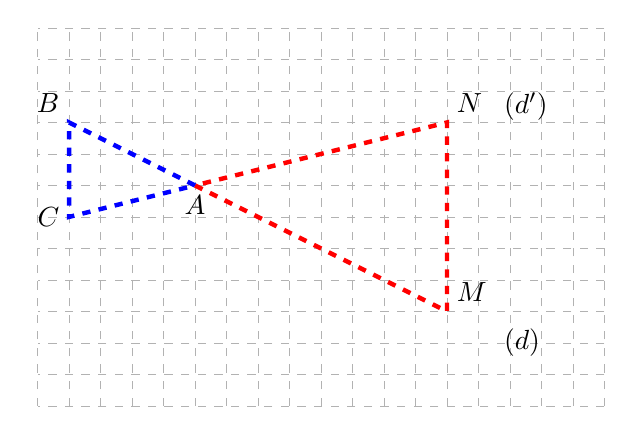
\begin{tikzpicture}[scale = 0.4]
                    \begin{scope}[rotate=90]
                    \draw[help lines, color=black!30, dashed] (0,0) grid (12,18);        
                    \coordinate[label=below:$A$] (A) at (7,13);
                    \coordinate[label=right:$(d')$] (d') at (9.5,3.5);
                    \coordinate[label=right:$(d)$] (d) at (2,3.5);
                    \coordinate[label=above right:$N$] (N) at (9,5);
                    \coordinate[label=above right:$M$] (M) at (3,5);
                    \coordinate[label=above left:$B$] (B) at (9,17);
                    \coordinate (M1) at (10,17);
                    \coordinate[label=left:$C$] (C) at (6,17);
                    \coordinate (N1) at (5,17);
        
                    \tkzDrawLine(A,M);
                    \tkzDrawLine(A,N);
                    \tkzDrawLine(M,N);
                    \tkzDrawLine(B,C);
                    \tkzDrawLine(M1,N1);     
                    \draw[dashed, color=red, ultra thick] (A)--(M)--(N)--(A);
                    \draw[dashed, color=blue, ultra thick] (A)--(B)--(C)--(A);
                    \end{scope}
                \end{tikzpicture}
            \end{minipage}
            \begin{minipage}{8cm}
                \begin{itemize}
                    \item Les droites $(d)$ et $(d')$ se coupent en $A$.
                    \item $AB=\Lg{5.4}$ ; $AM=\Lg{9}$.
                    \item $AC=\Lg{7.5}$ ; $AN=\Lg{12.5}$.
                \end{itemize}

                % \vspace*{1cm}
                Démontrer que les droites $(MN)$ et $(BC)$ sont parallèles.
            \end{minipage}
            
            \correction
            Dans la configuration ci-dessus : 
            \begin{itemize}
                \item les droites $(MB)$ et $(CN)$ sont sécantes en $A$.                
                \item les deux triangles de la configurations sont \textcolor{red}{$AMN$} et \textcolor{blue}{$ABC$}.
                \item Les points $A, M, B$ sont alignés dans le même ordre que les points $A, N, C$.
                \medskip
                \item D'une part $\dfrac{\textcolor{blue}{AB}}{\textcolor{red}{AM}} = \dfrac{\textcolor{blue}{5,4}}{\textcolor{red}{9}}=0,6$
                \hfill
                D'autre part $\dfrac{\textcolor{blue}{AC}}{\textcolor{red}{AN}} = \dfrac{\textcolor{blue}{7,5}}{\textcolor{red}{12,5}}=0,6$
            \end{itemize}
            On constate que $\dfrac{AM}{AB} = \dfrac{AN}{AC}$, d'après la réciproque du théorème de Thalès, on peut conclure que \psshadowbox{les droites $(MN)$ et $(BC)$ ne sont pas parallèles}.
        \end{methode*1}

% \subsection{Sous-section 1.1}
% \begin{definition}[Titre optionnel]
%     Dans le cours, on utilise assez souvent des cadres du type
%     définition (comme ici par exemple).    
% \end{definition}
% \begin{remarque}
%     Ceci est une remarque utilisant une commande du paquet profcollege.
    
%     \begin{center}
%       Truc centré
%     \end{center}


% \end{remarque}
% \begin{propriete}[Titre optionnel]
%   Dans le cours, on utilise assez souvent des cadres du type
%   définition, comme ici par exemple pour une propriete.
% \end{propriete}
% \begin{remarques}
%   \begin{itemize}
%     \item remarque.
%     \item remarque.
%   \end{itemize}
% \end{remarques}

% \subsection{Sous-section 1.2}
% \begin{theoreme}[Titre optionnel]
%   Dans le cours, on utilise assez souvent des cadres du type
%   définition, comme ici par exemple pour un théorème.
% \end{theoreme}
% \begin{notation}
%   notation
% \end{notation}
% \begin{notations}
%   \begin{itemize}
%     \item notation.
%     \item notation.
%   \end{itemize}
% \end{notations}
% \begin{preuve}
%   Ceci est une preuve\par Deuxième ligne de la preuve
% \end{preuve}
% \begin{exemple}
%   Texte de l’exemple
%   \correction
  
% \end{exemple}

% \begin{exemple*1}
%   \phantom{rrr}
%   Texte

%   \correction
%   \phantom{rrr}
%   Texte  
  
% \end{exemple*1}

% \begin{exemple}[0.6]
%   Texte de l’exemple très long sur une ligne, très très très long.
%   On peut modifier la répartition horizontale  à l'aide d'un argument optionnel valant par défaut 0,4, valant ici 0,6.
%   \correction
%   Texte de la correction en vis à vis
% \end{exemple}
% \section{Section 2}
% \subsection{Sous-section 2.1}
% Quatre affichages prévus pour les méthodes.

% \begin{methode}[Titre de la méthode]
%     \Papiers[Largeur=10,Hauteur=5,Couleur=Olive]
    
%     Texte introductif
%     \exercice
%     Texte de l’exercice
%     \correction
%     Texte de la correction sur un minimum de trois lignes pour faire la
%     différence entre vis-à-vis et double colonne. C’est l’endroit de la
%     coupure qui va différer.
% \end{methode}

% \begin{methode*1}[Titre de la méthode*1]
%     Texte introductif
%     \exercice
%     Texte de l’exercice
%     \correction
%     Texte de la correction sur un minimum de trois lignes pour faire la
%     différence entre vis-à-vis et double colonne. C’est l’endroit de la
%     coupure qui va différer.
% \end{methode*1}

% \subsection{Sous-section 2.2}
% \begin{methode*2}[Titre de la méthode*2]
%     Texte introductif
%     \exercice
%     Texte de l’exercice
%     \correction
%     Texte de la correction sur un minimum de trois lignes pour faire la
%     différence entre vis-à-vis et double colonne. C’est l’endroit de la
%     coupure qui va différer.
% \end{methode*2}

% \begin{methode*2*2}[Dernière méthode  \MethodeRefExercice{exoN1-exemple1} \MethodeRefExercice{exoN1-exemple2}]
%     \exercice
%     \label{methodeN1-exemple}
%     Texte du premier exercice
%     \correction
%     Correction du premier exercice
%     \exercice
%     Texte du deuxième exercice
%     \correction
%     Texte de la correction du deuxième exercice sur un minimum de trois
%     lignes pour faire la différence entre vis-à-vis et double
%     colonne. C’est l’endroit de la coupure qui va différer.
% \end{methode*2*2}